% Build: ./build.ps1 (PowerShell) or bash build.sh (macOS/Linux).
\documentclass[12pt,a4paper]{article}
\usepackage{fontspec}
\usepackage{polyglossia}
\setdefaultlanguage{russian}
\setotherlanguage{english}
\setmainfont{Times New Roman}
\setmonofont{Consolas}
\usepackage{amsmath,amssymb}
\usepackage{graphicx,booktabs,float}
\usepackage{geometry,setspace}
\usepackage{xcolor,listings}
\usepackage[unicode,hidelinks]{hyperref}
\geometry{left=25mm,right=20mm,top=20mm,bottom=20mm}
\onehalfspacing
\setlength{\parindent}{1.25cm}
\setlength{\emergencystretch}{2em}
\graphicspath{{figures/}}
\lstset{language=Python,basicstyle=\ttfamily\small,breaklines=true,
  frame=single,rulecolor=\color{black!20},columns=fullflexible,
  keepspaces=true,showstringspaces=false,tabsize=4,
  keywordstyle=\color{blue!45!black},commentstyle=\color{black!55}}
% Generated by lab3.py.
\newcommand{\TauMs}{0{,}250}
\newcommand{\TauGraphMs}{0{,}250000}
\newcommand{\HalfMs}{0{,}173287}
\newcommand{\HalfGraphMs}{0{,}173288}
\newcommand{\OmegaZero}{1054{,}093}
\newcommand{\FreqZero}{167{,}764}
\newcommand{\PeriodZeroMs}{5{,}960753}
\newcommand{\GammaBase}{138{,}889}
\newcommand{\OmegaDamped}{1044{,}902}
\newcommand{\PeriodDampedMs}{6{,}013179}
\newcommand{\PeriodNumericMs}{6{,}013179}
\newcommand{\PeriodIncrease}{0{,}8795}
\newcommand{\CriticalR}{379{,}473}
\newcommand{\FreeTimeEndMs}{36{,}079}
\newcommand{\QualityBase}{3{,}7947}
\newcommand{\WidthBase}{277{,}778}
\newcommand{\VoltageReactive}{37{,}947}
\newcommand{\MaxWidthErrorPercent}{0{,}00014}
\newcommand{\MaxPeakErrorPercent}{0{,}0000000}


\begin{document}
\begin{titlepage}
\begin{center}
\begin{spacing}{1.3}
\textbf{МИНИСТЕРСТВО ОБРАЗОВАНИЯ РЕСПУБЛИКИ БЕЛАРУСЬ}\\[0.25cm]
\textbf{БЕЛОРУССКИЙ ГОСУДАРСТВЕННЫЙ УНИВЕРСИТЕТ}\\[0.25cm]
\textbf{ФАКУЛЬТЕТ МЕХАНИКО-МАТЕМАТИЧЕСКИЙ}\\[0.25cm]
\textbf{Кафедра веб-технологий и компьютерного моделирования}
\end{spacing}
\vspace{4.2cm}
\textbf{ПЕРЕХОДНЫЕ И РЕЗОНАНСНЫЕ ПРОЦЕССЫ\\
В ЭЛЕКТРИЧЕСКИХ ЦЕПЯХ}\\[0.4cm]
Лабораторная работа № 3\\[0.2cm]
Вариант 4
\end{center}
\vspace{3.2cm}
\noindent\hspace*{0.48\textwidth}\begin{minipage}{0.52\textwidth}
\begin{spacing}{1.0}
Панасика Владислава Александровича\\
обучающегося 4 курса специальности\\
«Математика и компьютерные науки»\\[0.6cm]
Научный руководитель:\\
ассистент КФОиПИ,\\
Полякова Яна Владимировна
\end{spacing}
\end{minipage}
\vfill
\begin{center}Минск, 2026\end{center}
\end{titlepage}
\setcounter{page}{2}
\tableofcontents
\clearpage

\section*{Цель работы и исходные данные}
Исследовать переходные процессы в RC- и RLC-цепях и характеристики
электрического резонанса. Параметры варианта 4:
\[
R=50\ \text{Ом},\quad L=180\ \text{мГн}=0{,}18\ \text{Гн},\quad
C=5\ \text{мкФ}=5\cdot10^{-6}\ \text{Ф},\quad U_0=10\ \text{В}.
\]
В свободном режиме $q(0)=CU_0=50$ мкКл, $i(0)=0$.
При вынужденных колебаниях $u(t)=U_0\sin\omega t$.

\section{Задание 1. Разряд конденсатора в RC-цепи}
При положительном направлении тока разряда $i_{\mathrm{разр}}=-dq/dt$.
Из $i_{\mathrm{разр}}=U/R$ и $q=CU$ получаем
\begin{equation}
 RC\frac{dU}{dt}+U=0,\qquad
 U(t)=U_0e^{-t/(RC)}.
\end{equation}
Постоянная времени и время уменьшения напряжения вдвое:
\begin{equation}
 \tau=RC=\TauMs\ \text{мс},\qquad
 t_{1/2}=RC\ln2=\HalfMs\ \text{мс}.
\end{equation}
График построен на интервале $0\le t\le5RC=1{,}25$ мс.
Пересечения его дискретной ломаной с уровнями $U_0/e$ и $U_0/2$
найдены линейной интерполяцией:
\[
 t_{U_0/e}=\TauGraphMs\ \text{мс},\qquad
 t_{U_0/2}=\HalfGraphMs\ \text{мс}.
\]
Они согласуются с расчётными значениями. Здесь шаг графика равен
$1{,}25$ мкс, а при $t=5\tau$ остаётся $U=10e^{-5}\approx0{,}0674$ В.

\begin{figure}[H]
\centering
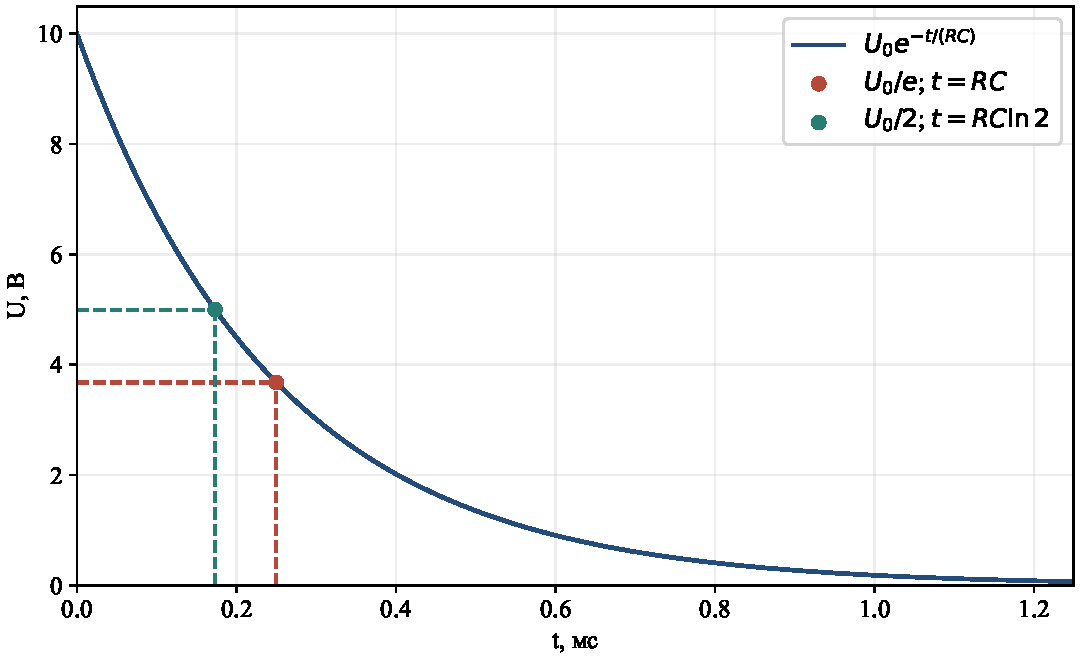
\includegraphics[width=0.72\textwidth]{task1_rc.pdf}
\caption{Разряд конденсатора и характерные уровни напряжения.}
\end{figure}

\clearpage
\section{Задание 2. Влияние параметров RC-цепи}
Для $R/2$, $R$ и $2R$ при неизменной ёмкости использовано
$U(t)=U_0e^{-t/(RC)}$. Результаты:
\begin{table}[H]
\centering
\caption{Характерные времена разряда при $C=5$ мкФ}
\begin{tabular}{rrr}
\toprule
$R$, Ом & $\tau$, мс & $t_{1/2}$, мс\\
\midrule
\input results/rc_rows.tex
\bottomrule
\end{tabular}
\end{table}
\begin{figure}[H]
\centering
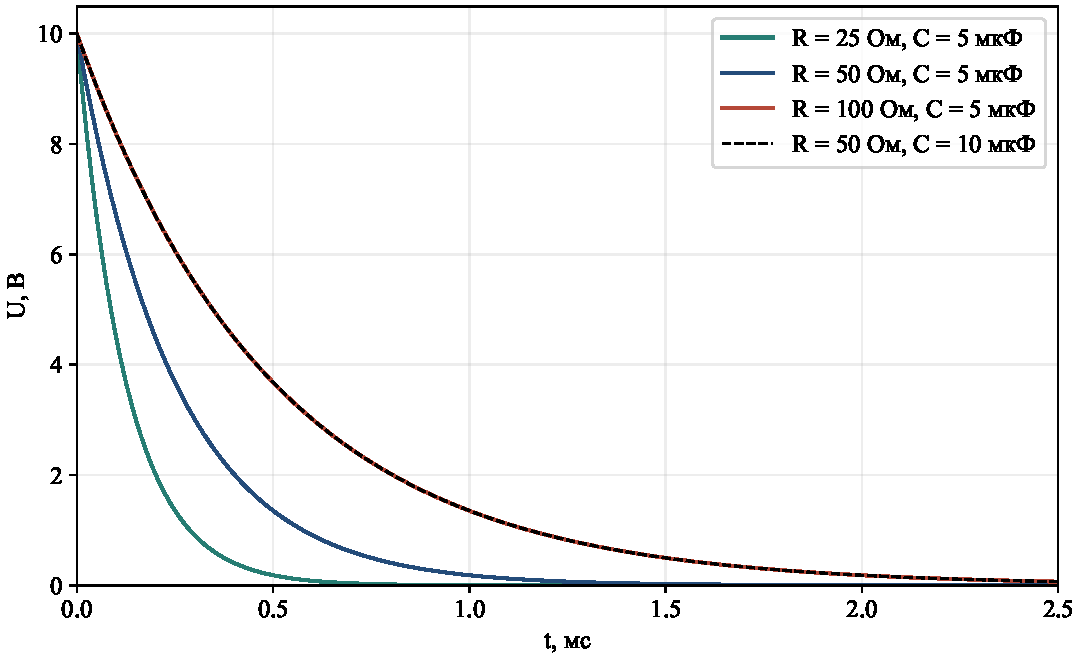
\includegraphics[width=0.88\textwidth]{task2_rc_parameters.pdf}
\caption{Влияние сопротивления и удвоения ёмкости на разряд.}
\end{figure}
Чем больше $R$, тем меньше начальный ток $U_0/R$ и медленнее разряд.
При увеличении $R$ вдвое постоянная времени также удваивается.
При $C'=2C=10$ мкФ и $R=50$ Ом
\[
 \tau'=R(2C)=2\tau=0{,}500\ \text{мс}.
\]
Поэтому кривые для $(R,2C)$ и $(2R,C)$ совпадают. Это равенство
проверено вычислением значений на общей временной сетке.
\begin{lstlisting}
t = np.linspace(0, 5 * (2 * R) * C, 2001)
for resistance in (R / 2, R, 2 * R):
    voltage = U0 * np.exp(-t / (resistance * C))
voltage_double_c = U0 * np.exp(-t / (R * 2 * C))
\end{lstlisting}

\clearpage
\section{Задание 3. Свободные колебания в RLC-цепи}
В свободном последовательном контуре по второму правилу Кирхгофа
\begin{equation}
 L\frac{di}{dt}+Ri+\frac qC=0.
\end{equation}
Здесь положительное направление тока выбрано по соглашению $i=dq/dt$.
Следовательно,
\begin{equation}
 Lq''+Rq'+\frac qC=0,\qquad q(0)=CU_0,\quad q'(0)=0.
 \label{eq:free}
\end{equation}
Для численного решения уравнение представлено системой:
\begin{equation}
 \begin{cases}
 \dot q=i,\\
 \dot i=-\dfrac RL i-\dfrac{1}{LC}q.
 \end{cases}
\end{equation}
Применён адаптивный метод DOP853 из \texttt{solve\_ivp}:
относительный допуск $10^{-10}$, абсолютные допуски
$10^{-14}$ Кл и $10^{-12}$ А; максимальный внутренний шаг $T_0/100$.
\begin{lstlisting}
def free_rhs(t, state, resistance):
    q, current = state
    return current, -(resistance * current + q / C) / L

solution = solve_ivp(
    free_rhs, (0, times[-1]), (C * U0, 0.0),
    args=(R,), method="DOP853", t_eval=times,
    rtol=1e-10, atol=(1e-14, 1e-12),
    max_step=T0 / 100, events=positive_maximum
)
\end{lstlisting}
Параметры колебаний:
\begin{align}
 \omega_0&=\frac1{\sqrt{LC}}=\OmegaZero\ \text{рад/с},
 &T_0&=2\pi\sqrt{LC}=\PeriodZeroMs\ \text{мс},\\
 \gamma&=\frac R{2L}=\GammaBase\ \text{с}^{-1},
 &\omega_d&=\sqrt{\omega_0^2-\gamma^2}=\OmegaDamped\ \text{рад/с},\\
 T_d&=\frac{2\pi}{\omega_d}=\PeriodDampedMs\ \text{мс}.
\end{align}
Для сверки использовано аналитическое решение:
\begin{align}
 q(t)&=CU_0e^{-\gamma t}
 \left[\cos(\omega_dt)+\frac{\gamma}{\omega_d}\sin(\omega_dt)\right],\\
 i(t)&=-CU_0\frac{\omega_0^2}{\omega_d}e^{-\gamma t}\sin(\omega_dt).
\end{align}

\begin{figure}[H]
\centering
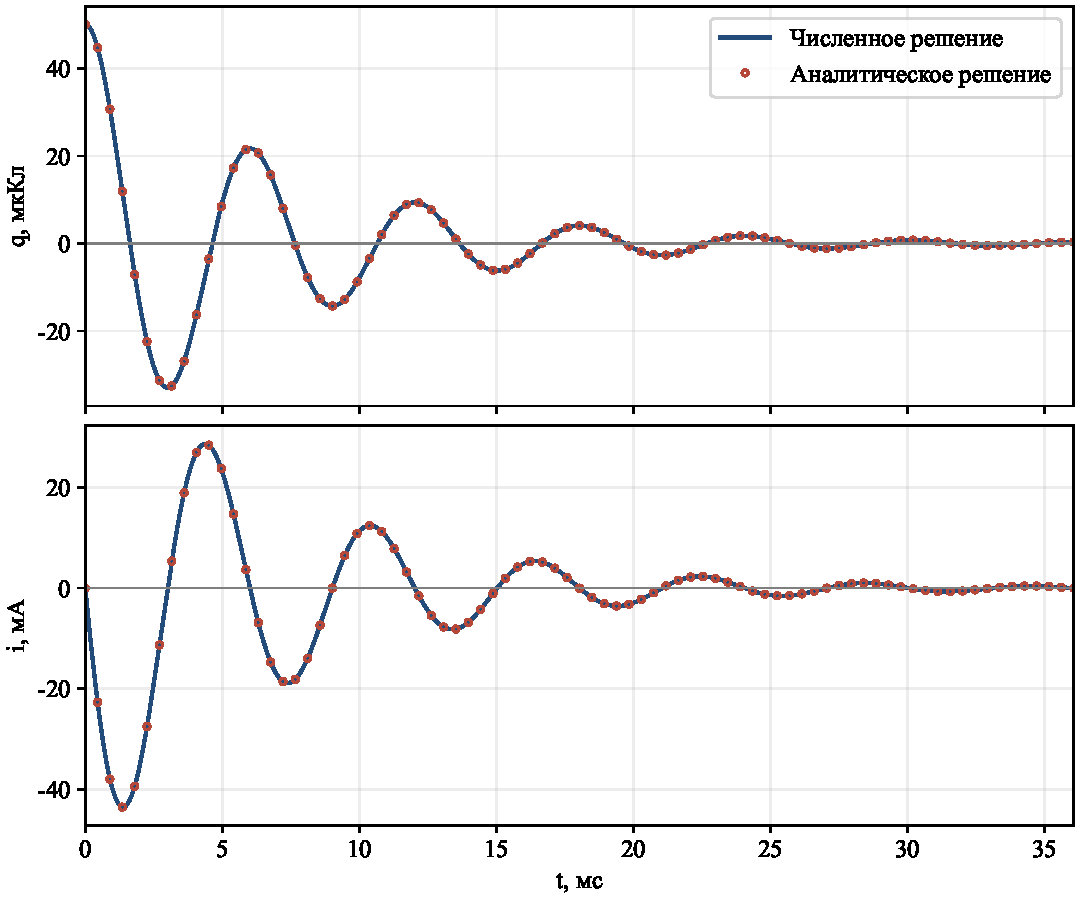
\includegraphics[width=0.94\textwidth]{task3_free.pdf}
\caption{Заряд и ток при свободных затухающих колебаниях, $R=50$ Ом.}
\end{figure}
Интервал моделирования $0\le t\le6T_d=\FreeTimeEndMs$ мс
превышает пять периодов $T_0$. Период по последовательным положительным
максимумам заряда, найденным как события $i=0$ с переходом от плюса к минусу:
\[
 T_{\mathrm{числ}}=\PeriodNumericMs\ \text{мс}.
\]
Он совпадает с $T_d$ в приведённых разрядах и превышает $T_0$ на
\PeriodIncrease\,\%. При $R>0$ в колебательном режиме
$\omega_d<\omega_0$, поэтому характерный период увеличивается.
Отрицательный ток в начале разряда обусловлен соглашением $i=dq/dt$:
заряд первоначально убывает.

Проверен энергетический баланс свободного контура:
\begin{equation}
 W(t)=\frac{q^2}{2C}+\frac{Li^2}{2},\qquad
 \frac{dW}{dt}=-Ri^2,\qquad W(0)=0{,}250\ \text{мДж}.
\end{equation}
Максимальные абсолютные отклонения численного решения от аналитического
меньше $10^{-12}$ Кл для заряда и $10^{-9}$ А для тока;
относительная невязка интегрального энергетического баланса меньше $10^{-6}$.

\clearpage
\section{Задание 4. Режимы затухания}
Корни характеристического уравнения~\eqref{eq:free} равны
$s_{1,2}=-\gamma\pm\sqrt{\gamma^2-\omega_0^2}$.
Критическое сопротивление определяется условием $\gamma=\omega_0$:
\begin{equation}
 R_{\mathrm{кр}}=2\sqrt{\frac LC}=\CriticalR\ \text{Ом}.
\end{equation}
При неизменных $L$ и $C$ численно рассчитаны три режима:
\begin{itemize}
 \item $R=0{,}5R_{\mathrm{кр}}\approx189{,}737$ Ом:
 комплексные корни, затухающие колебания со сменой знака заряда;
 \item $R=R_{\mathrm{кр}}\approx379{,}473$ Ом:
 кратный вещественный корень, критическое затухание;
 \item $R=2R_{\mathrm{кр}}\approx758{,}947$ Ом:
 два отрицательных вещественных корня, апериодический разряд.
\end{itemize}
Для проверки двух неколебательных режимов использованы формулы
\begin{align}
 q_{\mathrm{кр}}(t)&=CU_0(1+\omega_0t)e^{-\omega_0t},\\
 q_{\mathrm{ап}}(t)&=CU_0e^{-\gamma t}
 \left[\cosh(\kappa t)+\frac\gamma\kappa\sinh(\kappa t)\right],
 \qquad \kappa=\sqrt{\gamma^2-\omega_0^2}.
\end{align}
\begin{figure}[H]
\centering
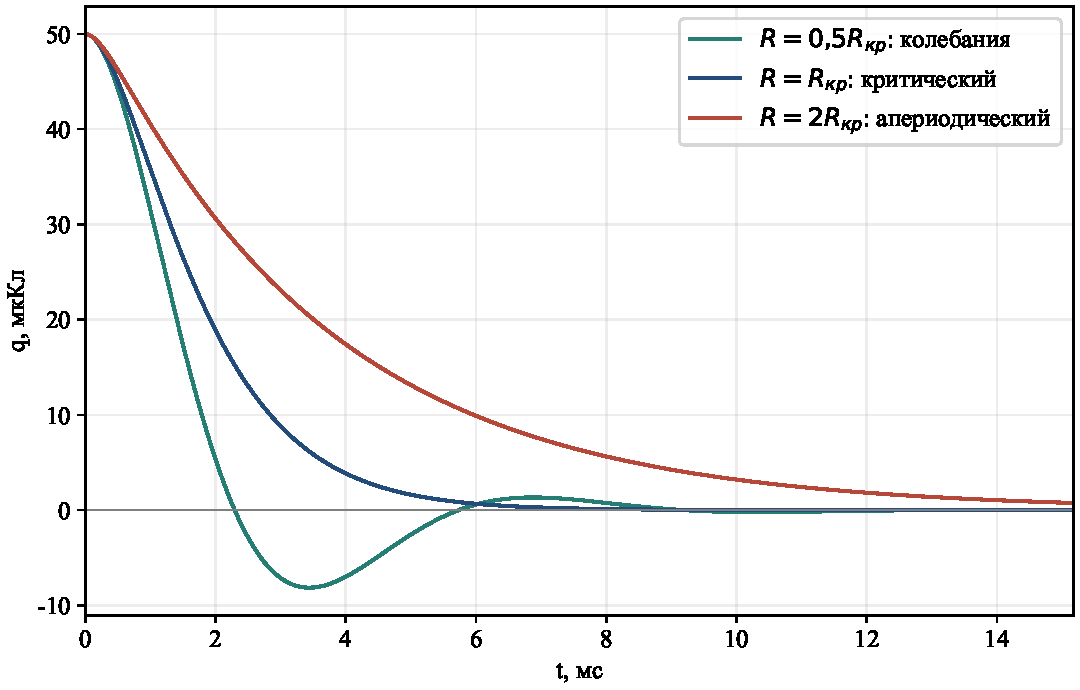
\includegraphics[width=0.77\textwidth]{task4_damping.pdf}
\caption{Три режима затухания при одинаковых начальных условиях.}
\end{figure}
В колебательном режиме энергия обменивается между электрическим и магнитным
полями, постепенно переходя в теплоту. Критический режим при заданных
начальных условиях даёт наиболее быстрое возвращение к равновесию без
смены знака заряда. При дальнейшем увеличении $R$ ток ограничивается
сильнее, и разряд становится более медленным.

\clearpage
\section{Задание 5. Резонанс в последовательной RLC-цепи}
Для источника $u(t)=U_0\sin\omega t$ уравнение имеет вид
\begin{equation}
 Lq''+Rq'+q/C=U_0\sin\omega t.
\end{equation}
После затухания переходной составляющей амплитуда установившегося тока:
\begin{equation}
 I_0(\omega)=\frac{U_0}{\sqrt{R^2+\left(\omega L-1/(\omega C)\right)^2}}.
 \label{eq:amplitude}
\end{equation}
Кривые рассчитаны в диапазоне
$0{,}4\omega_0\le\omega\le1{,}8\omega_0$ для $R=25$, 50 и 100 Ом.
Теоретический максимум возникает при компенсации реактивных сопротивлений:
\begin{equation}
 \omega_{\mathrm{рез}}=\omega_0=\OmegaZero\ \text{рад/с},\quad
 f_0=\frac{\omega_0}{2\pi}=\FreqZero\ \text{Гц},\quad
 I_{\max}=\frac{U_0}{R}.
\end{equation}
\begin{figure}[H]
\centering
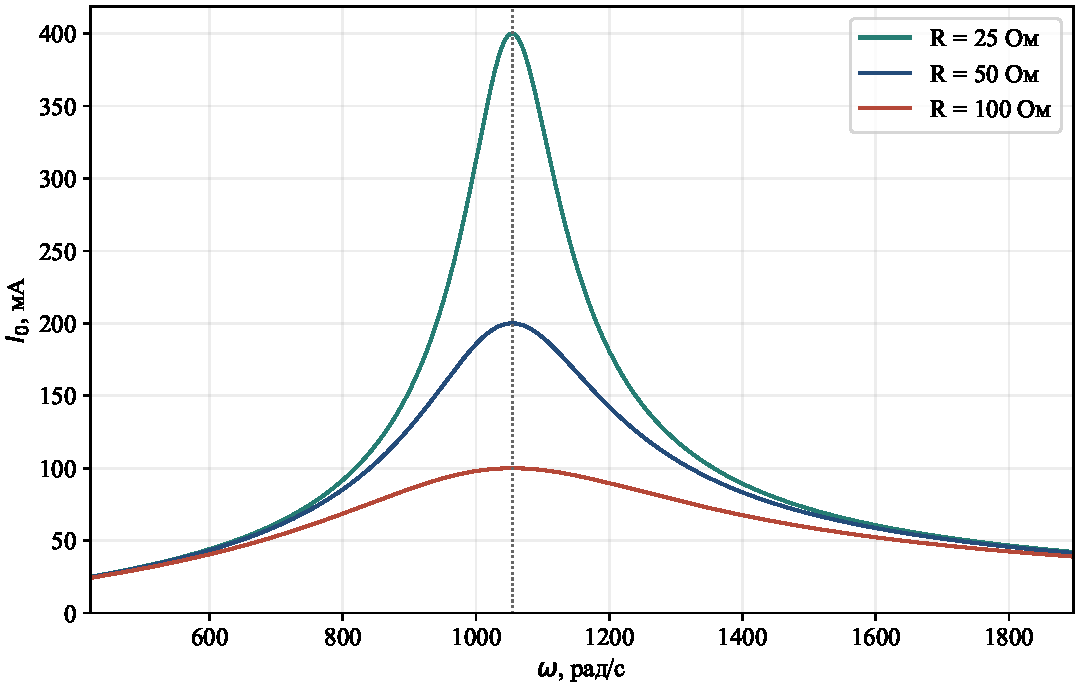
\includegraphics[width=0.74\textwidth]{task5_resonance.pdf}
\caption{Амплитудно-частотные характеристики при трёх сопротивлениях.}
\end{figure}
\begin{table}[H]
\centering
\caption{Численное определение максимума резонансных кривых}
\begin{tabular}{rrrr}
\toprule
$R$, Ом & $\omega_{\mathrm{сетка}}$, рад/с & $\omega_{\max}$, рад/с & $I_{\max}$, мА\\
\midrule
\input results/resonance_rows.tex
\bottomrule
\end{tabular}
\end{table}
На сетке использована 4001 точка; максимум уточнён минимизацией
$-I_0(\omega)$. Относительное отклонение уточнённой частоты от $\omega_0$
меньше $10^{-5}$. Уменьшение $R$ повышает максимум тока,
сохраняя его частоту $\omega_0$.

\clearpage
\section{Задание 6. Фазочастотная характеристика}
Принято соглашение $\varphi=\varphi_U-\varphi_I$. Тогда
\begin{equation}
 \varphi(\omega)=\operatorname{atan2}
 \left(\omega L-\frac1{\omega C},R\right),\qquad
 i(t)=I_0\sin(\omega t-\varphi).
\end{equation}
\begin{figure}[H]
\centering
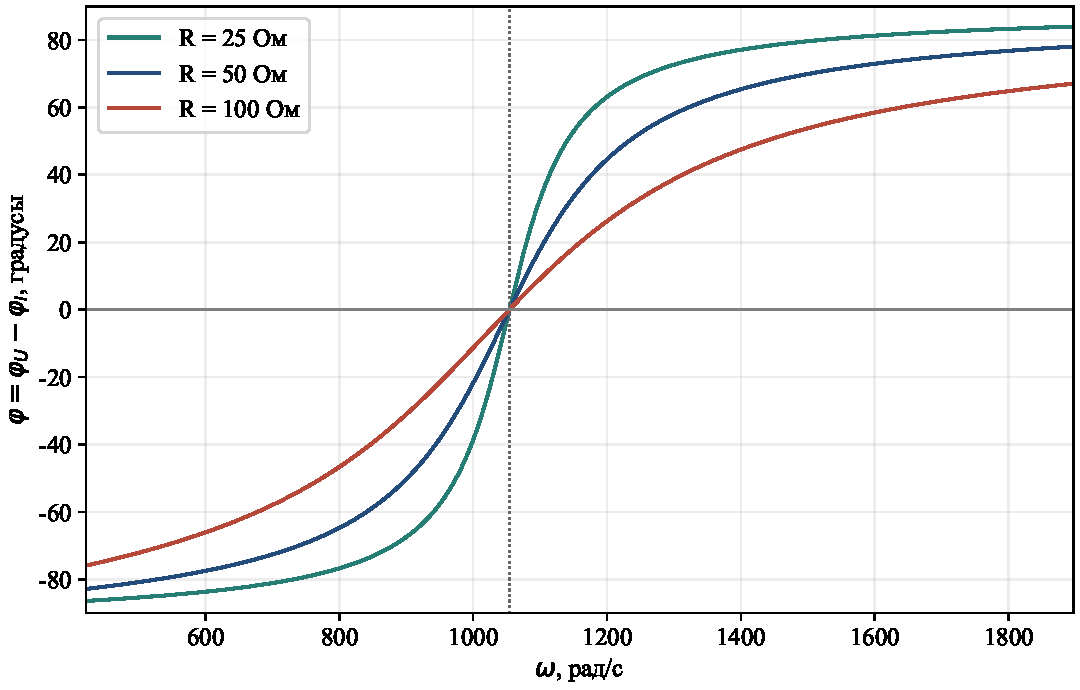
\includegraphics[width=0.92\textwidth]{task6_phase.pdf}
\caption{Фазочастотные характеристики; на графике фаза дана в градусах.}
\end{figure}
При $\omega<\omega_0$ имеем $X_C>X_L$, $\varphi<0$:
ток опережает напряжение. При $\omega>\omega_0$ имеем
$X_L>X_C$, $\varphi>0$: ток отстаёт от напряжения.
При $\omega=\omega_0$ реактивная часть равна нулю,
и ток совпадает с напряжением по фазе. Эти границы одинаковы
для всех трёх сопротивлений.
\begin{lstlisting}
phi = np.arctan2(omega * L - 1 / (omega * C), R)
phi_degrees = np.rad2deg(phi)
\end{lstlisting}
Изменение $R$ влияет на крутизну фазовой характеристики:
меньшему сопротивлению соответствует более резкий переход около резонанса.

\clearpage
\section{Задание 7. Добротность и ширина резонанса}
Добротность последовательного контура:
\begin{equation}
 Q=\frac{\omega_0L}{R}=\frac1R\sqrt{\frac LC}.
\end{equation}
Частоты половинной мощности определяются уровнем
$I_0(\omega_{1,2})=I_{\max}/\sqrt2$. Из~\eqref{eq:amplitude}
следует $|\omega L-1/(\omega C)|=R$, поэтому
\begin{align}
 \omega_{1,2}&=\sqrt{\omega_0^2+\left(\frac R{2L}\right)^2}\mp\frac R{2L},\\
 \Delta\omega&=\omega_2-\omega_1=\frac RL,\qquad Q=\frac{\omega_0}{\Delta\omega}.
\end{align}
Численные границы найдены линейной интерполяцией точек графика
на уровне $I_{\max}/\sqrt2$.
\begin{figure}[H]
\centering
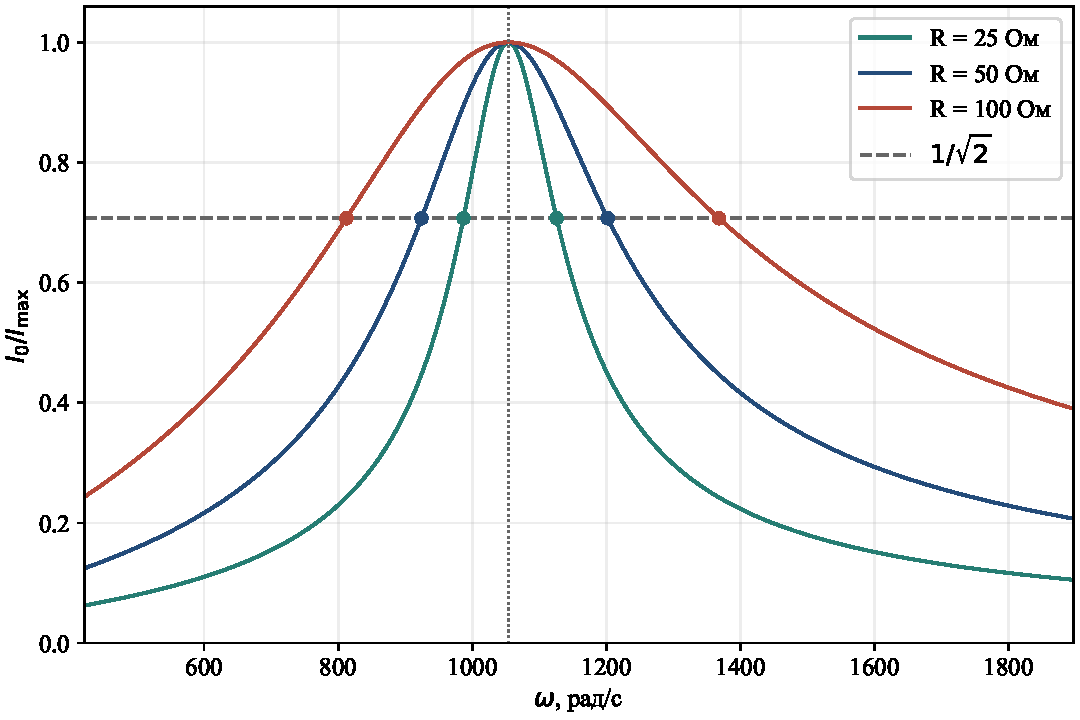
\includegraphics[width=0.70\textwidth]{task7_bandwidth.pdf}
\caption{Нормированные резонансные кривые и точки половинной мощности.}
\end{figure}
\begin{table}[H]
\centering
\caption{Добротность и границы полосы; все частоты в рад/с}
\begin{tabular}{rrrrrr}
\toprule
$R$, Ом & $Q$ & $\omega_{1,\mathrm{числ}}$ & $\omega_{2,\mathrm{числ}}$
& $\Delta\omega_{\mathrm{числ}}$ & $R/L$\\
\midrule
\input results/bandwidth_rows.tex
\bottomrule
\end{tabular}
\end{table}
Максимальное относительное расхождение ширины, определённой по графику,
с $R/L$ составляет \MaxWidthErrorPercent\,\% и связано с дискретизацией.
Обе границы находятся внутри заданного диапазона частот для всех трёх $R$.
Уменьшение $R$ вдвое удваивает добротность и вдвое сужает полосу;
при увеличении $R$ вдвое наблюдается обратный эффект.

\clearpage
\section{Ответы на контрольные вопросы}
\subsection*{1. Что определяет постоянная времени RC-цепи?}
Постоянная времени $\tau=RC$ задаёт скорость экспоненциального
переходного процесса. При разряде за это время напряжение уменьшается
в $e$ раз. При заряде через резистор отклонение от установившегося
напряжения уменьшается в $e$ раз.

\subsection*{2. Как получить уравнение свободных колебаний RLC-цепи?}
По второму правилу Кирхгофа в свободном последовательном контуре
$U_L+U_R+U_C=0$. Подставляя $U_L=L\,di/dt$, $U_R=Ri$,
$U_C=q/C$ и выбирая $i=dq/dt$, получаем
$Lq''+Rq'+q/C=0$. В этой работе заданы $q(0)=CU_0$, $q'(0)=0$.

\subsection*{3. Как сопротивление влияет на характер затухания?}
Коэффициент затухания $\gamma=R/(2L)$ растёт с сопротивлением.
При $R<R_{\mathrm{кр}}=2\sqrt{L/C}$ процесс колебательный,
при равенстве --- критический, при превышении --- апериодический.
В колебательном режиме увеличение $R$ усиливает затухание и уменьшает
частоту $\omega_d$. При очень большом $R$ разряд становится медленнее,
поскольку ток через конденсатор ограничен сопротивлением.

\subsection*{4. При каком условии возникает резонанс напряжений?}
В последовательной цепи условие резонанса $X_L=X_C$, то есть
$\omega L=1/(\omega C)$ и $\omega=\omega_0=1/\sqrt{LC}$.
Полное сопротивление становится равным $R$, ток максимален и совпадает
по фазе с напряжением источника. Напряжения катушки и конденсатора равны
по амплитуде и противоположны по фазе; каждое имеет амплитуду $QU_0$.
Для варианта 4 это $\VoltageReactive$ В при амплитуде источника 10 В.

\subsection*{5. Почему фазовый сдвиг меняет знак при резонансе?}
Реактивное сопротивление $X=\omega L-1/(\omega C)$ монотонно
возрастает с частотой и меняет знак в точке $\omega_0$.
Ниже резонанса цепь имеет ёмкостный характер, выше --- индуктивный.
При выбранном соглашении $\varphi_U-\varphi_I$ это означает переход
от отрицательной фазы к положительной через ноль.

\subsection*{6. Что характеризует добротность и как она связана с шириной?}
Добротность $Q=\omega_0L/R$ характеризует остроту резонанса
и относительную величину потерь. При резонансе она равна отношению
амплитуды напряжения на катушке или конденсаторе к амплитуде источника.
Поскольку $\Delta\omega=R/L$, имеем $Q=\omega_0/\Delta\omega$:
чем выше добротность, тем уже полоса.

\section*{Вывод}
Для варианта 4 получена постоянная времени RC-цепи
$\tau=\TauMs$ мс и время уменьшения напряжения вдвое
$t_{1/2}=\HalfMs$ мс. Удвоение сопротивления или ёмкости удваивает
постоянную времени. Численное решение свободных колебаний согласуется
с аналитическим; период $T_d=\PeriodDampedMs$ мс превышает
$T_0=\PeriodZeroMs$ мс. Найдено критическое сопротивление
$R_{\mathrm{кр}}=\CriticalR$ Ом и воспроизведены три режима затухания.

Частота максимального установившегося тока равна
$\omega_0=\OmegaZero$ рад/с ($f_0=\FreqZero$ Гц).
При её прохождении ток переходит от опережения напряжения к отставанию.
Для $R=50$ Ом получены $Q=\QualityBase$ и
$\Delta\omega=\WidthBase$ рад/с. Численные границы половинной мощности
согласуются с $\Delta\omega=R/L$: уменьшение сопротивления повышает
добротность и сужает полосу резонанса.
\end{document}
